	\documentclass[notitlepage, 11pt]{report}
	\usepackage[utf8]{inputenc}
	\usepackage{titling}
	\usepackage{amsmath}
	\usepackage{relsize}
	\usepackage{breqn}
	\usepackage{graphicx}
	\usepackage{wrapfig}
	\usepackage{caption,subcaption}
	\usepackage{longtable}
	\usepackage{float}
	\usepackage{wrapfig,lipsum,booktabs}
	\graphicspath{ {./images/} }
	\setlength{\droptitle}{-5em}   % This is your set screw
	\usepackage[a4paper, total={7in, 10in}]{geometry}
	\title{Report \\
		\large{SPS Coursework: An Unknown Signal} \\
	}

	\author{Emil Centiu, zl18810}
	\begin{document}
		
		\maketitle	
		\renewcommand{\thesection}{\arabic{section}}

		\section{Least Squares Regression}
		
		\paragraph*{}	
		Because we can't assume anything about the random error term (i.e. follows a normal distribution like that in MLE), Least Squares Method was the go-to method to find the best fitting line. 
		
		The goal is to deterministicaly minimise the sum of squared differences between the observed value of the dependent variable ($ y_{i} $) and the predicted value of the dependent variable ($ \hat{y} $), that is provided by the regression function. In other words, we need to find $a, b$ so that the residual error $R(a, b)$ is minimised, where
		
		\begin{equation*}
			R(a, b) = \sum_{i=1}^{N}(\hat{y_{i}} - y_{i})^2 = 	\sum_{i=1}^{N}((a + bx_i) - y_i)^2
		\end{equation*}
		
		We can observe that $ R(a, b) $ plots as an eliptic paraboloid, so there is only one critical point, and according to Fermat's Theorem, there is a local extreme, hence the minimum value of the function. To find the pair $(a, b)$, we can just calculate the critical point out of the partial derivatives with respect to each variable:
		
		\begin{equation*}
			\dfrac{\delta{} R}{\delta{} a} = 	\dfrac{\delta{}}{\delta{} a} \sum_{i=1}^{N}(y_i^2 + a^2 + 2abx_i + b^2x^2 - 2y_ia - 2y_ibx_i)^2
			= \sum_{i=1}^{N}(2a + 2bx_i - 2y_i) = -2\sum_{i=1}^{N}(y_i - (a+bx_i)) = 0
		\end{equation*}
		\begin{equation*}
			\dfrac{\delta{} R}{\delta{} b} =\dfrac{\delta{}}{\delta{} b} \sum_{i=1}^{N}(y_i^2 + a^2 + 2abx_i + b^2x^2 - 2y_ia - 2y_ibx_i)^2 
			= \sum_{i=1}^{N}(2ax_i + 2bx_i^2 - 2y_ix_i) = -2\sum_{i=1}^{N}x_i(y_i - (a + bx_i)) = 0
		\end{equation*}
		
		Out of the first equation, we can get $a$:
		\begin{multline*}
			-2\sum_{i=1}^{N}(y_i - (a+bx_i)) = 0 \Leftrightarrow \sum_{i=1}^{N}y_i - Na + b \sum_{i=1}^{N}b_i = 0 \Leftrightarrow
			 a = \dfrac{\sum_{i=1}^{N}y_i - b \sum_{i=1}^{N}x_i }{N} \Leftrightarrow a = \overline{y} - b \overline{x} 
		\end{multline*}
		
		where $\overline{x}$ is the mean value of the $x$ coordinates, and $\overline{y}$, the mean value of the $y$ coordinates. An interesting observation is that the regression function always goes through the centroid (the point of coordinates $(\overline{x}, \overline{y})$).
		
		We can get $b$ out of the second equation, by substituting the value of $a$:		
		\begin{multline*}
			-2\sum_{i=1}^{N} x_i(y_i - (a+bx_i)) = 0 \Leftrightarrow 		\sum_{i=1}^{N}x_i(y_i -a - bx_i) = 0 \Leftrightarrow \sum_{i=1}^{N}x_iy_i - \sum_{i=1}^{N} x_ia - \sum_{i=1}^{N} x_i^2b = 0 \\
			\Leftrightarrow \sum_{i=1}^{N} x_iy_i - \sum_{i=1}^{N}x_i(\overline{y} - b\overline{x}) - \sum_{i=1}^{N} x_i^2b = 0 \Leftrightarrow \sum_{i=1}^{N}x_iy_i - \overline{y}\sum_{i=1}^{N}x_i + b\overline{x}\sum_{i=1}^{N}x_i - b\sum_{i=1}^{N} x_i^2 = 0 \\
			\Leftrightarrow \sum_{i=1}^{N} x_iy_i - \overline{y}N\overline{x} + N\overline{x}^2 - b\sum_{i=1}^{N}x_i^2 = 0 \Leftrightarrow b = \dfrac{\sum_{i=1}^{N}x_iy_i - N \overline{x}\overline{y}}{\sum_{i-1}^{N}x_i^2 - N\overline{x}^2}
 		\end{multline*}

		Now, this works only for linear functions, but a very interesting observation is that it will work the same way with vectors and matrices in place of $x$ and $y$, which will give us the possibility for more complex functions (polynomial for example):
 			
		\begin{multline*}
			R(a, b) = \sum_{i=1}^{N}(\hat{y_{i}} - y_{i})^2 = 	\sum_{i=1}^{N}((a + bx_i) - y_i)^2 = || y - Xa||^2$, where y$= \begin{bmatrix} y_1 \\ ... \\ y_N\end{bmatrix} $, x = $\begin{bmatrix} 1 & x_1 \\ ... \\ 1 & x_N\end{bmatrix} $ and a=$\begin{bmatrix} a \\ b\end{bmatrix}
		\end{multline*}
		Therefore, we need to calculate the matrix $a$:
		\begin{equation*}
			|| y - Xa||^2 = 0 \Rightarrow y-Xa = 0 \Rightarrow Xa = y \Rightarrow X^TXa = X^Ty \Rightarrow a = (X^TX)^{-1}X^Ty
		\end{equation*}
		
		\section{Figures/plots}
		
			\begin{figure}[H]
				\centering % <-- added
				\begin{subfigure}{0.25\textwidth}
					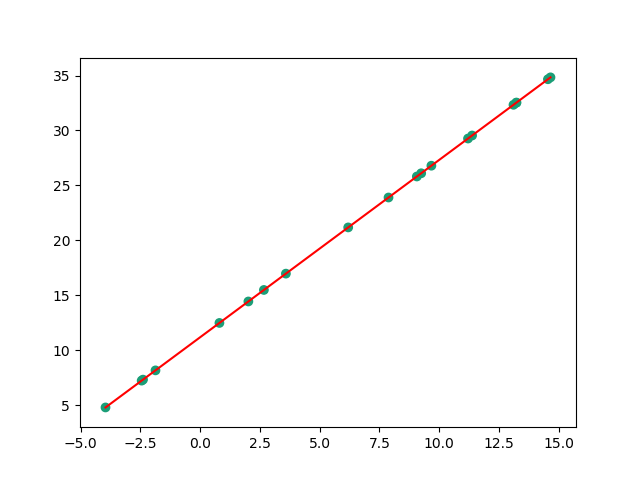
\includegraphics[width=\linewidth]{Figure_1}
					\caption{basic\_1}
					\label{fig:1}
				\end{subfigure}\hfil % <-- added
				\begin{subfigure}{0.25\textwidth}
					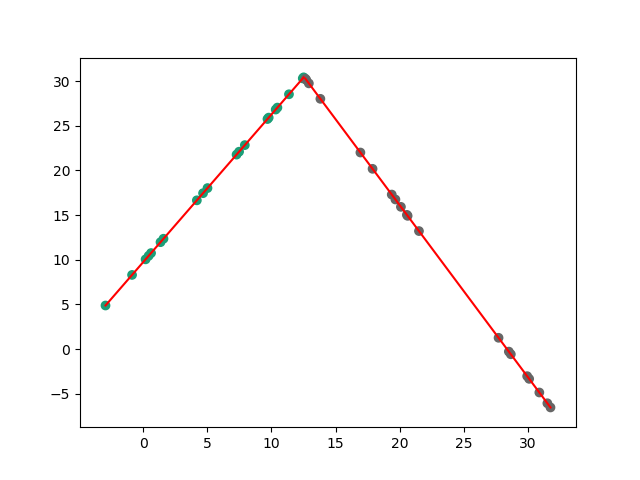
\includegraphics[width=\linewidth]{Figure_2}
					\caption{basic\_2}
					\label{fig:2}
				\end{subfigure}\hfil % <-- added
				\begin{subfigure}{0.25\textwidth}
					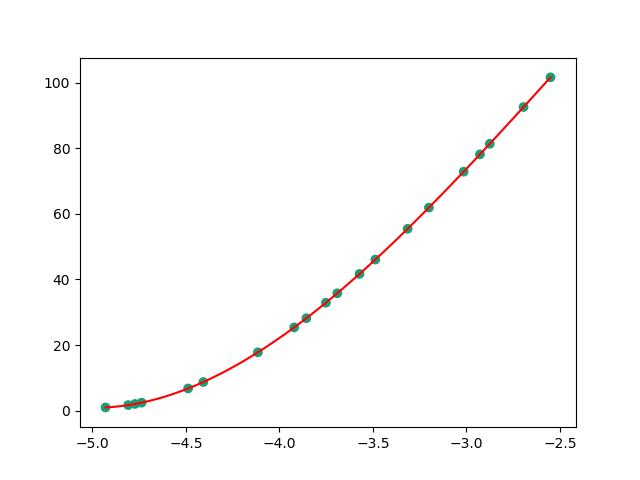
\includegraphics[width=\linewidth]{Figure_3}
					\caption{basic\_3}
					\label{fig:3}
				\end{subfigure}
				
				\medskip
				\begin{subfigure}{0.25\textwidth}
					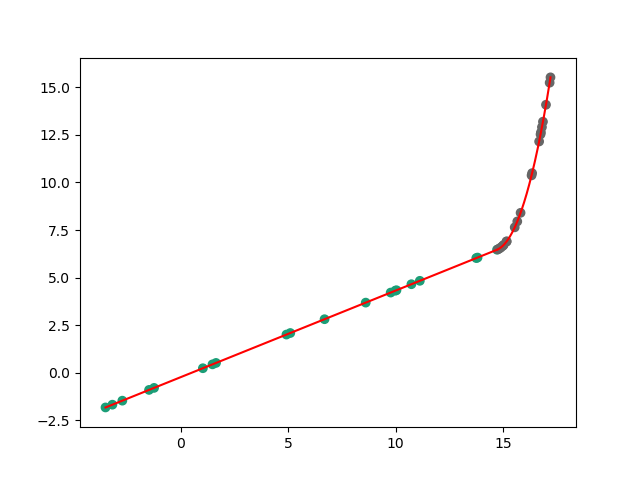
\includegraphics[width=\linewidth]{Figure_4}
					\caption{basic\_4}
					\label{fig:4}
				\end{subfigure}\hfil % <-- added
				\begin{subfigure}{0.25\textwidth}
					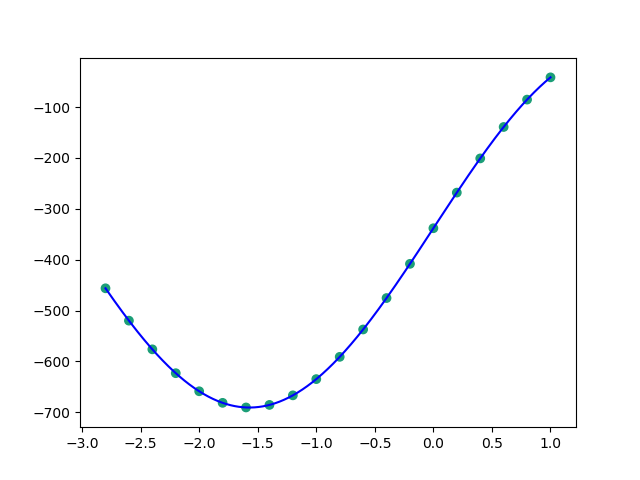
\includegraphics[width=\linewidth]{Figure_5}
					\caption{basic\_5}
					\label{fig:5}
				\end{subfigure}\hfil % <-- added
				\begin{subfigure}{0.25\textwidth}
					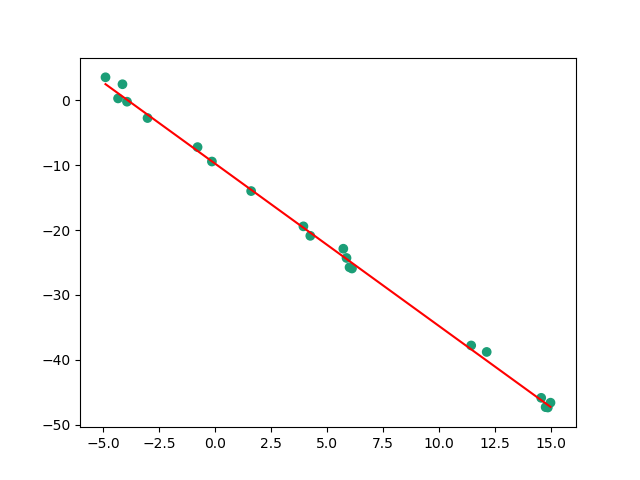
\includegraphics[width=\linewidth]{Figure_6}
					\caption{noise\_1}
					\label{fig:6}
				\end{subfigure}
			
				\medskip
				\begin{subfigure}{0.25\textwidth}
					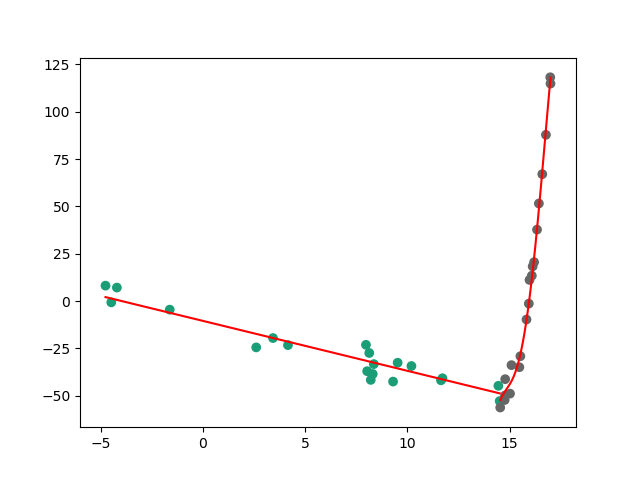
\includegraphics[width=\linewidth]{Figure_7}
					\caption{noise\_2}
					\label{fig:7}
				\end{subfigure}\hfil % <-- added
				\begin{subfigure}{0.25\textwidth}
					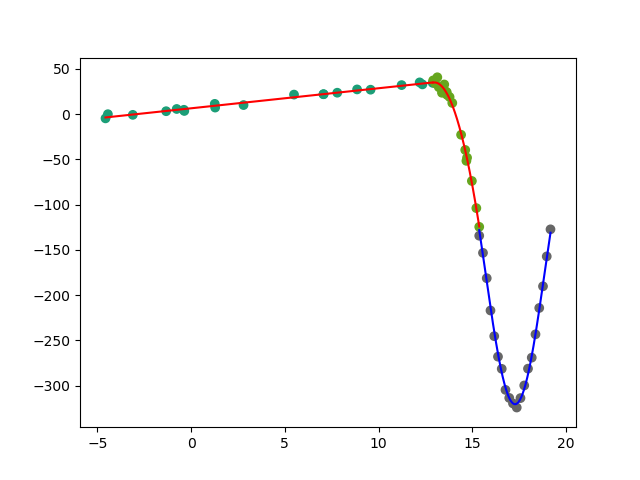
\includegraphics[width=\linewidth]{Figure_8}
					\caption{noise\_3}
					\label{fig:8}
				\end{subfigure}\hfil % <-- added
				\begin{subfigure}{0.25\textwidth}
					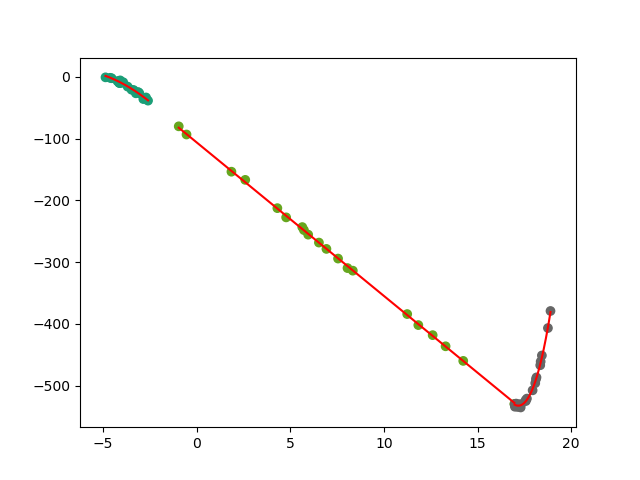
\includegraphics[width=\linewidth]{Figure_9}
					\caption{adv\_1}
					\label{fig:9}
				\end{subfigure}
					
			
				\medskip
				\begin{subfigure}{0.25\textwidth}
					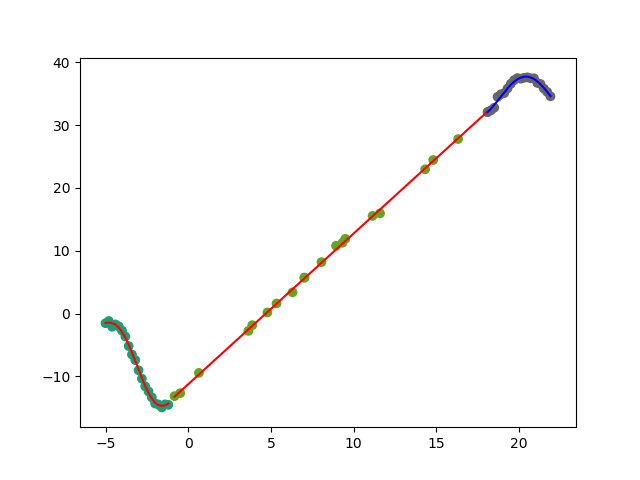
\includegraphics[width=\linewidth]{Figure_10}
					\caption{adv\_2}
					\label{fig:10}
				\end{subfigure}\hfil % <-- added
				\begin{subfigure}{0.25\textwidth}
					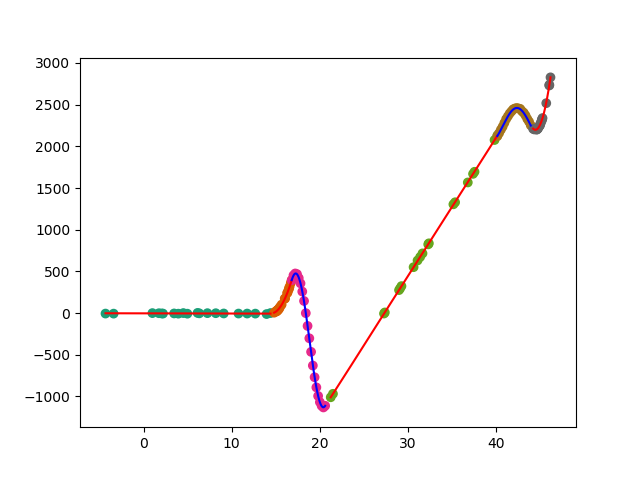
\includegraphics[width=\linewidth]{Figure_11}
					\caption{adv\_3}
					\label{fig:11}
				\end{subfigure}\hfil % <-- added
		
				
			
				\caption{Plots demonstrating the results for the training data provided}
				\label{fig:images}
			\end{figure}
		
				
		\section{Results Analysis}
				
		
		

			
			{
				\def\arraystretch{1.5}
			\begin{longtable}{ | c | c | }
				\hline
				training dataset & error\\ [1ex]
				\hline
				basic\_1.csv & 2.21354370005016e-27 \\ 
				\hline
				basic\_2.csv & 2.2.09284798155134e-27 \\
				\hline
				basic\_3.csv & 2.98184889123001e-17 \\
				\hline
				basic\_4.csv & 2.925811326716107e-11 \\
				\hline
				basic\_5.csv & 2.49608212186412e-25 \\
				\hline
				noise\_1.csv & 12.6404829302961 \\
				\hline
				noise\_2.csv & 832.929938008537 \\
				\hline
				noise\_3.csv & 485.12675214856 \\
				\hline
				adv\_1.csv & 210.706307324207 \\
				\hline
				adv\_2.csv & 3.57810739681056 \\
				\hline
				adv\_3.csv & 1020.48071055932 \\
				\hline
			\end{longtable}
		}

	
	\paragraph{Results}
	As expected, the basic training data gives very small errors, ranging from $10^{-27}$ to $10^{-11}$, as the data doesn't have much noise (almost none). The program has no problem whatsoever fitting the correct function.
	
	However, the noisier it is, the more likely it is to overfit. To prevent overfitting, especially on the noise sets, the program splits the data into training and testing, 3 points being allocated to testing, and the rest of them to training. This solution tremendously helped in combating the overfitting problem, as well as deciding the grade of the polynomial function. As a result, the program is capable of fitting any polynomial function (from linear to $6^{th}$ grade) without any problems. 
	
	Splitting the data into training and testing yielded higher errors, as there is less data to train on, but I think it is a good trade off when it comes to new data and generalisation. 
	
	Another problem I ran into was that of the constant functions ($y = 0*x + b$), in the sense that the program would fit the trigonometric functions instead of the constant ones because of noise. To solve this issue, I introduced a threshold value, so, for example, if the error is 0.01 greater with polynomial function than any trigonometric function, it will choose the polynomial instead.
	
	\paragraph{Implementation}
	I opted for an Object Oriented Design and combining it with the flexibility of the Least Squares Method allowed me to easily implement a variety of functions. For now, those functions are: $polynomial$, $cosine$, $sine$, $exponential$ and $logarithm$. Each function has its own class which contains functions to calculate the least squares matrix, to calculate the error, and to plot the fitted line. The main reasons I chose this modular design are: readability and maintainability of the code, and possible future extensions (i.e. more complicated functions that may even not use the least squares method).
	
	\section{Conclusion}
	\paragraph*{}
	All in all, I really enjoyed this assignment, it gave me a little glimpse of what data science really is. It gave me much better understanding of the Least Squares Method and helped me learn how to deal with overfitting and various tradeoffs.
		
	\end{document}